\ylDisplay{Kondensaatorid} % Ülesande nimi
{Mihkel Kree} % Autor
{lõppvoor} % Voor
{2009} % Aasta
{G 3} % Ülesande nr.
{6} % Raskustase
{
% Teema: Elektriahelad
\ifStatement
Koosnegu kondensaatorite süsteem viiest kondensaatorist. Alghetkel on kolm neist laenguta ning kahel paikneb laeng $q$ (vt joonist). Missugune laeng koguneb keskmisele kondensaatorile, kui süsteem on jõudnud tasakaaluolekusse?

\begin{center}
	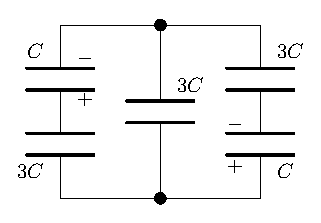
\includegraphics[width=0.42\linewidth]{2009-v3g-03-G_kondensaatorid.eps}
\end{center}
\fi


\ifHint
Süsteemis kehtib laengu jäävus, st alamsüsteemis, mis koosneb ülemisest sõlmpunktist ja sellega ühendatud kolmest kondensaatori plaadist peab alati olema summaarse laenguga $-q$. See kehtib sellepärast, et laengud saavad liikuda ainult mööda metalli ning ei saa eelmainitud alamsüsteemist õhu kaudu lahkuda.
\fi


\ifSolution
Kogunegu keskmisele kondensaatorile (mahtuvusega $3C$) laeng $a$ ning nurgas paiknevatele kondensaatoritele (mahtuvusega $3C$) laeng $b$. Vaatleme ülemist vasakpoolset kondensaatorit: selle negatiivsel plaadil on nüüd laeng $-q+a+b$ ning positiivsel plaadil $q+b$. Saame võrrandi:
\[-(-q+a+b)=q+b \implies q-a-b=q+b \implies b=-a/2.\]
Lisaks saame pingete võrdsusest
\[\frac{a}{3C}=\frac{q+b}{C}+\frac{b}{3C}\implies a=3q+4b\implies a+2a=3q,\]
millest $a=q$.
\fi
}